\newpage
\section{ILP --- Static Parallelism}
\subsection{Instruction-Level Parallelism(ILP)}

\subsubsection{Basic Pipeline}
An implementation technique
whereby multiple instructions are
overlapped in execution
\subsubsection{Data Hazard \& Forwarding}
The hazard detection by comparing the destination and sources of adjacent instructions

\subsection{floating-point pipeline}
\subsubsection{Multicycle FP Operation}
allow for a longer latency for op, i.e. take >1 cc for EXE. 

Two changes over integer pipeline:
\begin{enumerate}
    \item repeat EX
    \item use multiple FP functional units. e.g. FP adder, FP divider
\end{enumerate}
\begin{figure}[!htb]
    \centering
    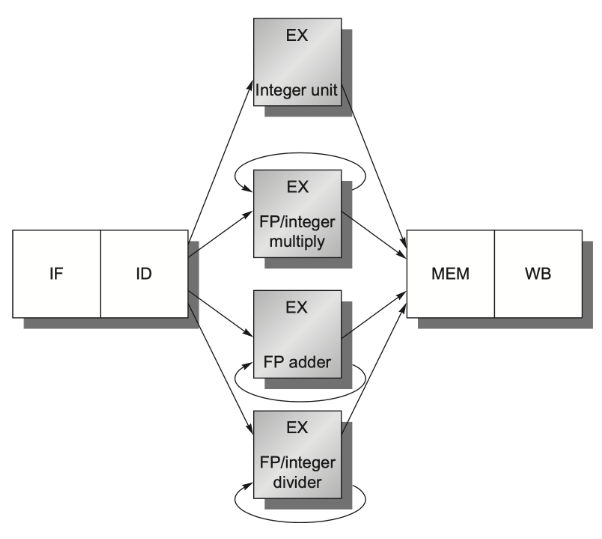
\includegraphics[width=0.309\textwidth]{pic/CA3/FP Pipeline}
    \caption{FP Pipeline}
\end{figure}

EX is not pipelined

\subsubsection{Latency \& Ini/Repeat Interval}
\begin{itemize}\small
    \item Latency: the number of intervening cycles
    between an instruction that produces a
    result and an instruction that uses the
    result
    \item Initiation/Repeat Interval: the number of cycles that must elapse
    between issuing two operations of a
    given type
\end{itemize}
\begin{table}[!htb]
    \centering
    \caption{Latency \& Ini/Repeat Interval}
    \begin{tabular}[c]{lcc}\toprule
        \textbf{Functional unit} & \textbf{Latency} & \textbf{Initiation interval} \\ \midrule
        Integer ALU         & 0 & 1 \\
        FP/integer loads    & 1 & 1 \\
        FP add              & 3 & 1 \\
        FP/integer multiply & 6 & 1 \\
        FP/integer divide   & 24 & 25 \\
        \bottomrule
    \end{tabular}
\end{table}
% \begin{figure}[!htb]
%     \centering
%     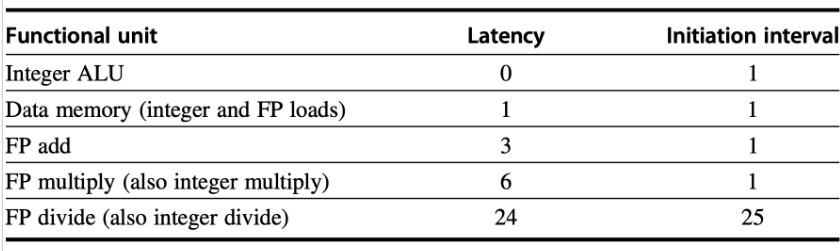
\includegraphics[width=0.42\textwidth]{pic/CA3/latency.png}
%     \caption{Latency \& Ini/Repeat Interval}
% \end{figure}


\subsubsection{Generalized FP Pipeline}
EX is pipelined (except for FP divider). with Additional pipeline registers
\begin{figure}[!htb]
    \centering
    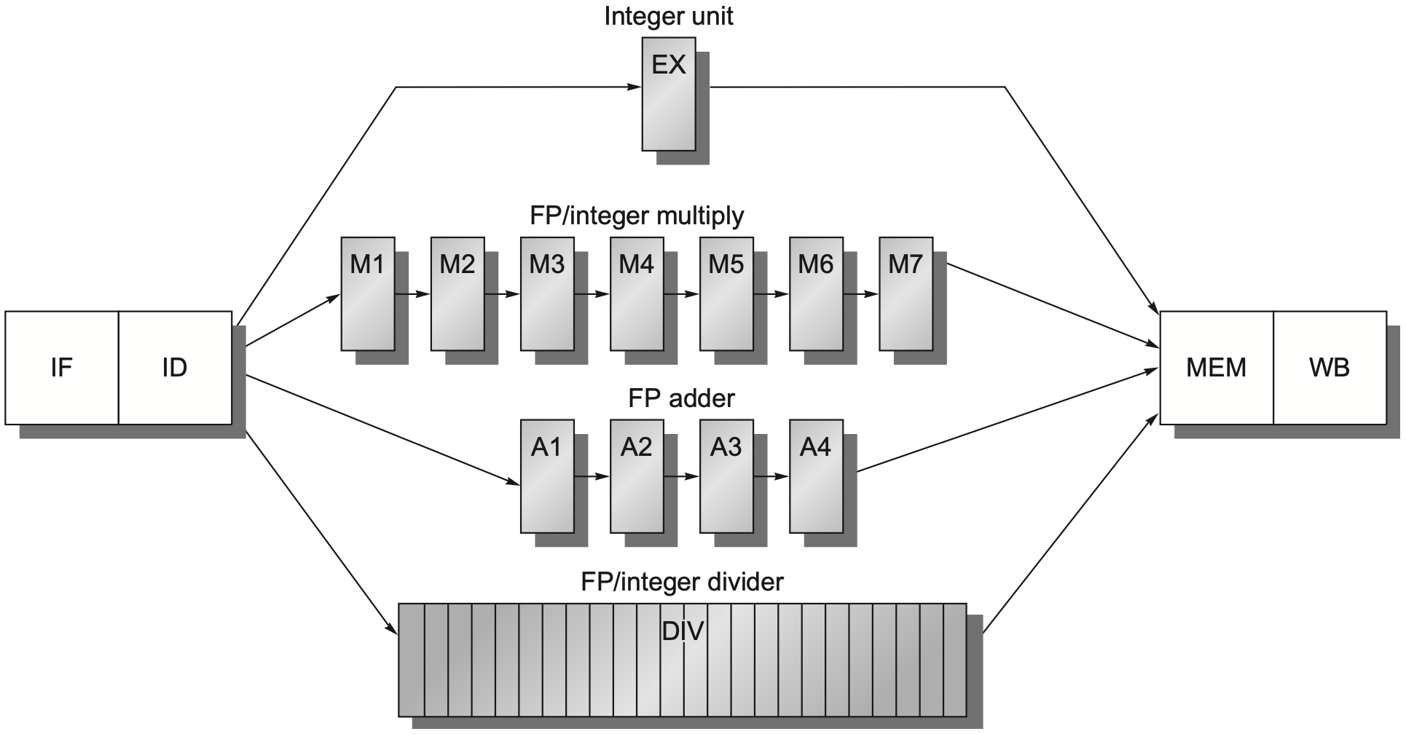
\includegraphics[width=0.42\textwidth]{pic/CA3/Generalized FP Pipeline}
    \caption{Generalized FP Pipeline}
\end{figure}
但因为每条指令长度不一样, 会有乱序的问题. 

\subsection{FP pipeline hazards}
\subsubsection{Structural Hazard}
Instructions have varying running
times, maybe $>1$ register write in a
cycle. 

Solution: Interlock Detection. 

\subsubsection{WAW Hazard}
Write after write (WAW) hazard: Instructions no longer reach WB in order.

Solution:
\begin{enumerate}
    \item delay issuing
    \item zero write control
\end{enumerate}

\subsubsection{RAW Hazard}
Longer latency of operations,  more frequent stalls for
read after write (RAW) hazards

\subsubsection{Hazard: Exceptions}
Instructions may complete in a different order than they were issued – exceptions

\subsubsection{Forwarding}

Generalized with more sources EX/MEM, A4/MEM, M7/MEM, D/MEM, MEM/WB -> source registers of an FP instruction. 


\subsubsection{Out-of-Order Completion}
How to deal with out-of-order:
\begin{enumerate}
    \item ignore the problem
    \item buffer the results of an operation
    until all the operations issued earlier
    complete
    \item track what operations were in the
    pipeline and their PCs for trap-handling
    \item issue an instruction only if it is
    certain that all previous instructions
    will complete without exception
\end{enumerate}

\subsection{ILP Exploitation}
\begin{itemize}
    \item Compiler-based static parallelism
    \item Hardware-based dynamic parallelism
\end{itemize}


\subsection{Static Scheduling}
\begin{itemize}
    \item Pipeline Scheduling
    \item Loop Unrolling
\end{itemize}

\subsubsection{Pipeline Scheduling}
e.g. 
\begin{minted}{c++}
    for(i=999;i>=0;i-=1) x[i]=x[i]+s;
\end{minted}

\begin{minted}{asm}
Loop:
    fld    f0, 0(x1)
    fadd.d f4, f0, f2
    fsd    f4, 0(x1)
    addi   x1, x1, -8
    bne    x1, x2, Loop
\end{minted}
8 clock cycles per loop

\begin{minted}{asm}
Loop:
    fld    f0, 0(x1)
    addi   x1, x1, -8
    fadd.d f4, f0, f2
    fsd    f4, 8(x1)
    bne    x1, x2, Loop
\end{minted}
7 clock cycles per loop

loop overhead

\subsubsection{Loop Unrolling}
Replicate loop body multiple times given the same amount of overhead instructions
\begin{minted}{asm}
Loop:
    fld    f0, 0(x1)
    fadd.d f4, f0, f2
    fsd    f4, 0(x1) //drop addi & bne
    fld    f6, -8(x1)
    fadd.d f8, f6, f2
    fsd    f8, -8(x1) //drop addi & bne
    fld    f0, -16(x1)
    fadd.d f12, f0, f2
    fsd    f12, -16(x1) //drop addi & bne
    fld    f14, -24(x1)
    fadd.d f16, f14, f2
    fsd    f16, -24(x1)
    addi   x1, x1, -32
    bne    x1, x2, Loop
\end{minted}
26-CC per four ops

\subsubsection{Loop Unrolling \& Scheduling}
\begin{minted}{asm}
Loop:
    fld    f0, 0(x1)
    fld    f6, -8(x1)
    fld    f0, -16(x1)
    fld    f14, -24(x1)
    fadd.d f4, f0, f2
    fadd.d f8, f6, f2
    fadd.d f12, f0, f2
    fadd.d f16, f14, f2
    fsd    f4, 0(x1) 
    fsd    f8, -8(x1)
    fsd    f12, -16(x1)
    fsd    f16, -24(x1)
    addi   x1, x1, -32
    bne    x1, x2, Loop
\end{minted}

14-CC per four ops

\subsection{Handle Branches}
\begin{figure}[!htb]
    \centering
    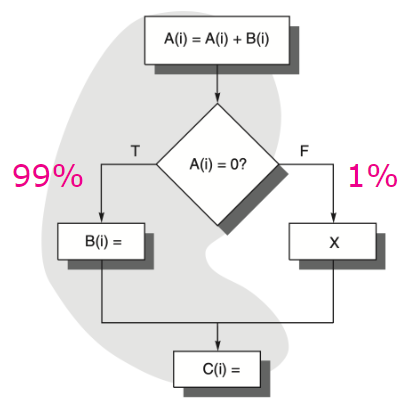
\includegraphics[width=0.309\textwidth]{pic/CA3/Frequent Critical Path}
    \caption{Frequent Critical Path}
\end{figure}
Focus on a frequent critical path as if the branch were gone

\subsubsection{Trace Scheduling}
Trace: a likely sequence of basic
blocks whose operations will be put
together into a smaller number of
instructions

\begin{itemize}
    \item Trace Selection: find the frequent path
    \item Trace Compaction: compress on-path instructions
    into fewer wider instructions
\end{itemize}
\begin{figure}[!htb]
    \centering
    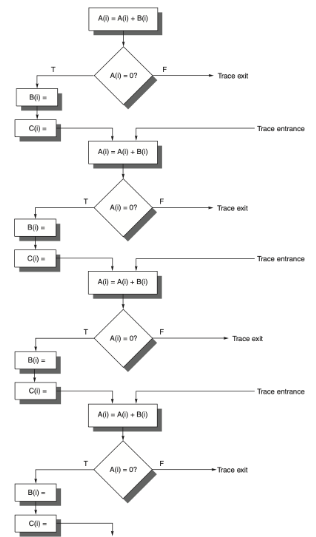
\includegraphics[width=0.22\textwidth]{pic/CA3/unrolled trace}
    \caption{unrolled trace}
\end{figure}

\begin{itemize}
    \item trace exit
    \item trace entrance
\end{itemize}
too many entrances and exits amidst the trace

\paragraph{Superblock}
\begin{figure}[!htb]
    \centering
    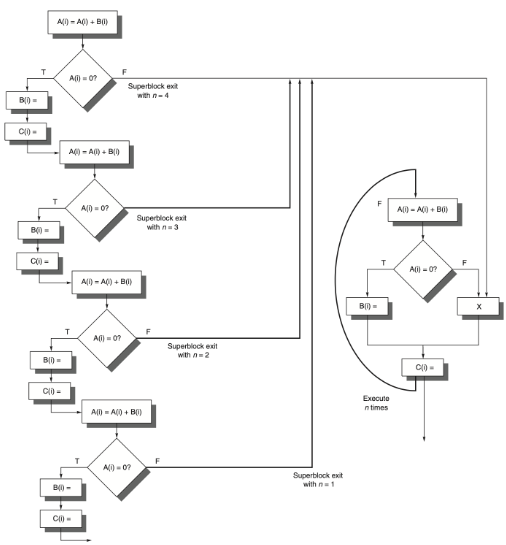
\includegraphics[width=0.309\textwidth]{pic/CA3/Superblock}
    \caption{Superblock}
\end{figure}
single entrance \& multiple exits

\paragraph{Fixup Code}
\begin{figure}[!htb]
    \centering
    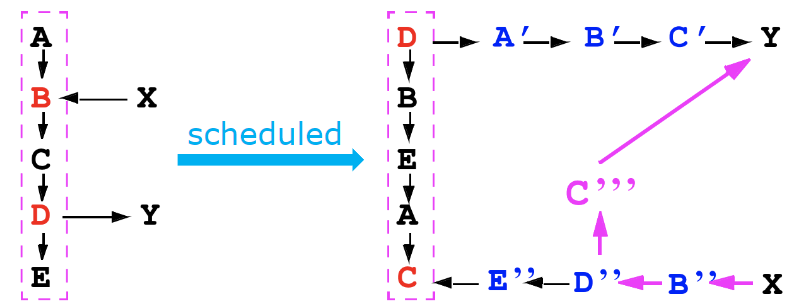
\includegraphics[width=0.42\textwidth]{pic/CA3/Fixup Code}
    \caption{Fixup Code/Compensation Code}
\end{figure}
copy instructions to ensure correctness of all paths

\subsubsection{Branch Hazard}
a branch may or may mot change PC to other values other than PC+4.

If the branch is untaken, the stall is unnecessary. 

Solutions: 4 simple compile time schemes
\begin{enumerate}
    \item Freeze or flush the pipeline: hold or delete any instructions after the
    branch till the branch dst is known
    \item Predicted-untaken / not-taken: simply treat every branch as untaken
    \item Predicted-taken: simply treat every branch as taken
    \item Delayed branch: delay the branch execution after the
    next instruction
\end{enumerate}

\newpage
\section{ILP --- Dynamic Parallelism}

\subsection{Static Branch Prediction}
\begin{figure}[!htb]
    \centering
    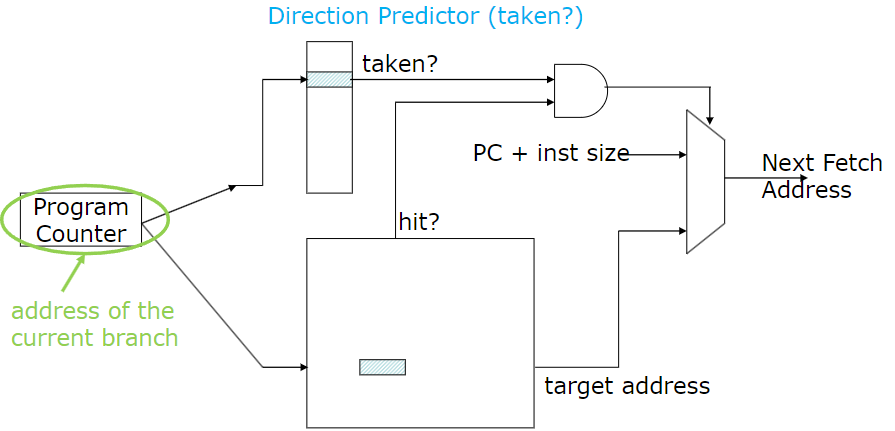
\includegraphics[width=0.42\textwidth]{pic/CA3/Static Branch Prediction}
    \caption{Static Branch Prediction}
\end{figure}

使用历史数据结合现在的指令进行判断, 会得到下一个预测的地址. 
\subsection{Dynamic Branch Prediction}
\begin{itemize}
    \item Follow branch history of taken branch
    \item Use branch prediction buffer (or BHT: branch history table) indexed by lower portion of branch address and marked with a bit to track taken/untaken status
\end{itemize}

\subsubsection{1,2,N-bit Predictor}
\begin{figure}[!htb]
    \centering
    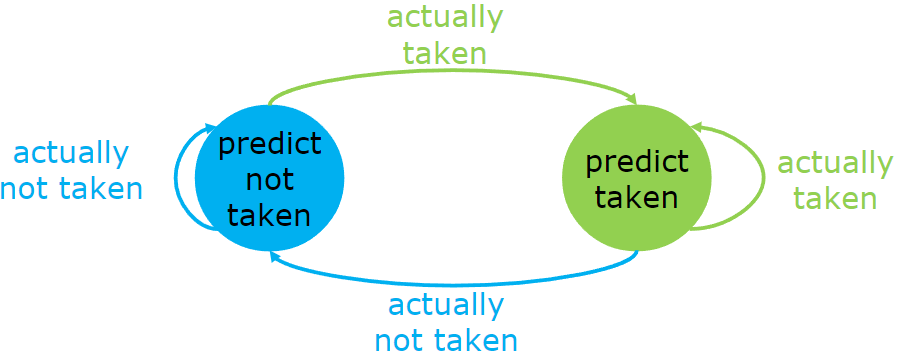
\includegraphics[width=0.42\textwidth]{pic/CA3/1-bit Predictor}
    \caption{1-bit Predictor}
\end{figure}

\begin{figure}[!htb]
    \centering
    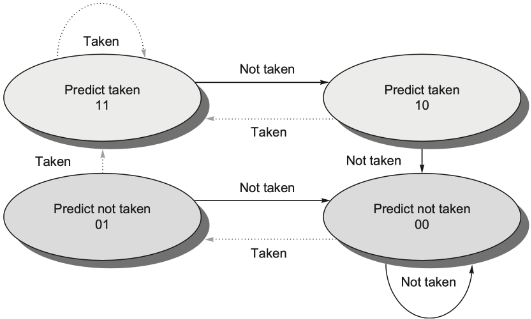
\includegraphics[width=0.42\textwidth]{pic/CA3/2-bit Predictor}
    \caption{2-bit Predictor}
\end{figure}

N-bit Predictor: assign an N-bit predictor per branch, range from $0$ to $2^N - 1$. Counter threshold: $\frac{2^N-1}{2}$.
\begin{itemize}
    \item greater: taken
    \item smaller: untaken
\end{itemize}

\subsubsection{Local Predictor} 
A branch's outcome can be correlated with past outcomes of the same branch (other than the outcome of the branch ``last-time'' it was executed). 即使用最近的历史进行预测. 

\begin{figure}[!htb]
    \centering
    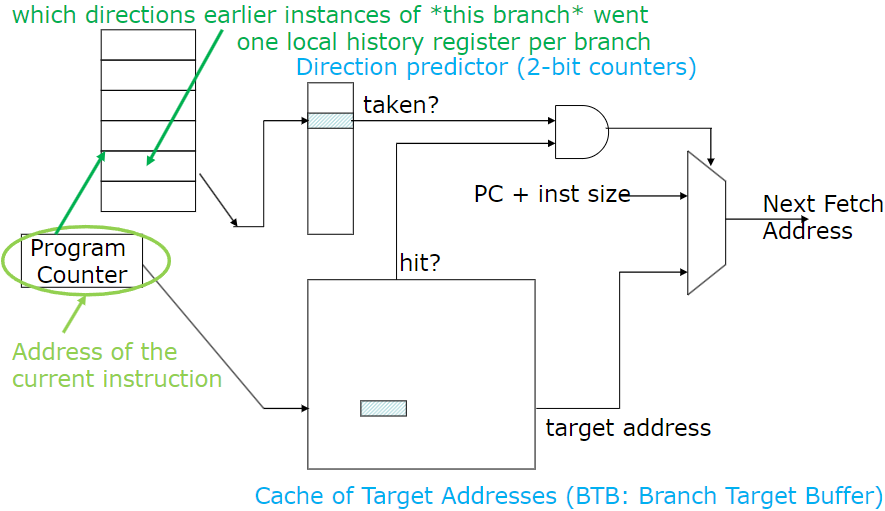
\includegraphics[width=0.42\textwidth]{pic/CA3/Local Predictor}
    \caption{Local Predictor}
\end{figure}

\subsection{Correlate Branch Prediction}
\subsubsection{Correlating/Two-level Predictor}
use the behavior of other branches to make a prediction.

\begin{figure}[!htb]
    \centering
    \includegraphics[width=0.42\textwidth]{pic/CA3/Two-level Predictor}
    \caption{Two-level Predictor}
\end{figure}

$(m, n)$ predictor: 
\begin{itemize}
    \item use the behavior of the last $m$ branches to choose from $2^m$ branch predictors, each predictor is an $n$-bit counter. 
    \item storage cost per branch given an individual pattern history table (PHT, $2^m\times n$ bits)
\end{itemize}

\subsubsection{Hybrid/Alloyed Predictor}
Use more than one type of predictor, Use more than one type of predictor.
\begin{figure}[!htb]
    \centering
    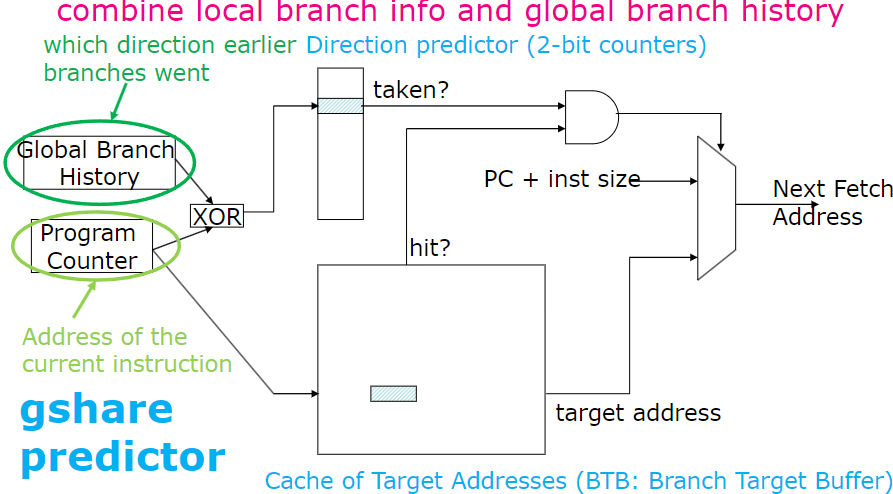
\includegraphics[width=0.42\textwidth]{pic/CA3/Hybrid Predictor}
    \caption{Hybrid/Alloyed Predictor}
\end{figure}

\subsubsection{Tournament Predictor}
\begin{itemize}
    \item Global predictor + Local predictor
    \item Choose either with a selector
\end{itemize}

\subsubsection{Tagged Hybrid Predictor}
Use a series of global predictors indexed with different length histories

\subsection{Dynamic Scheduling}
hardware reorders the instruction execution to reduce the stalls while maintaining data flow and exception behavior

\begin{itemize}
    \item Enable out-of-order execution
    \item Split ID into two stages:
    \begin{itemize}
        \item Issue: decode instructions, check for structural hazards
        \item Read operands: wait until no data hazards, then read operands
    \end{itemize}
\end{itemize}

Scheduling policy: upon stalling instruction, issue other instructions if they do not depend on any active or stalled instruction. 

How to schedule: use a centralized hazard detection and resolution unit

\subsubsection{Scoreboarding}
\begin{figure}[!htb]
    \centering
    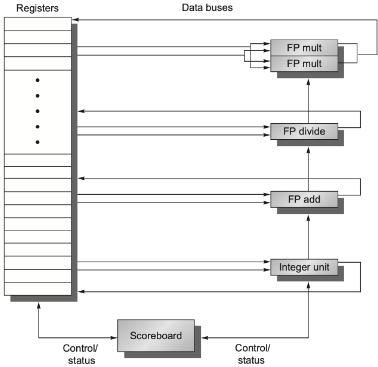
\includegraphics[width=0.309\textwidth]{pic/CA3/Scoreboarding}
    \caption{Scoreboarding}
\end{figure}

\begin{figure}[!htb]
    \centering
    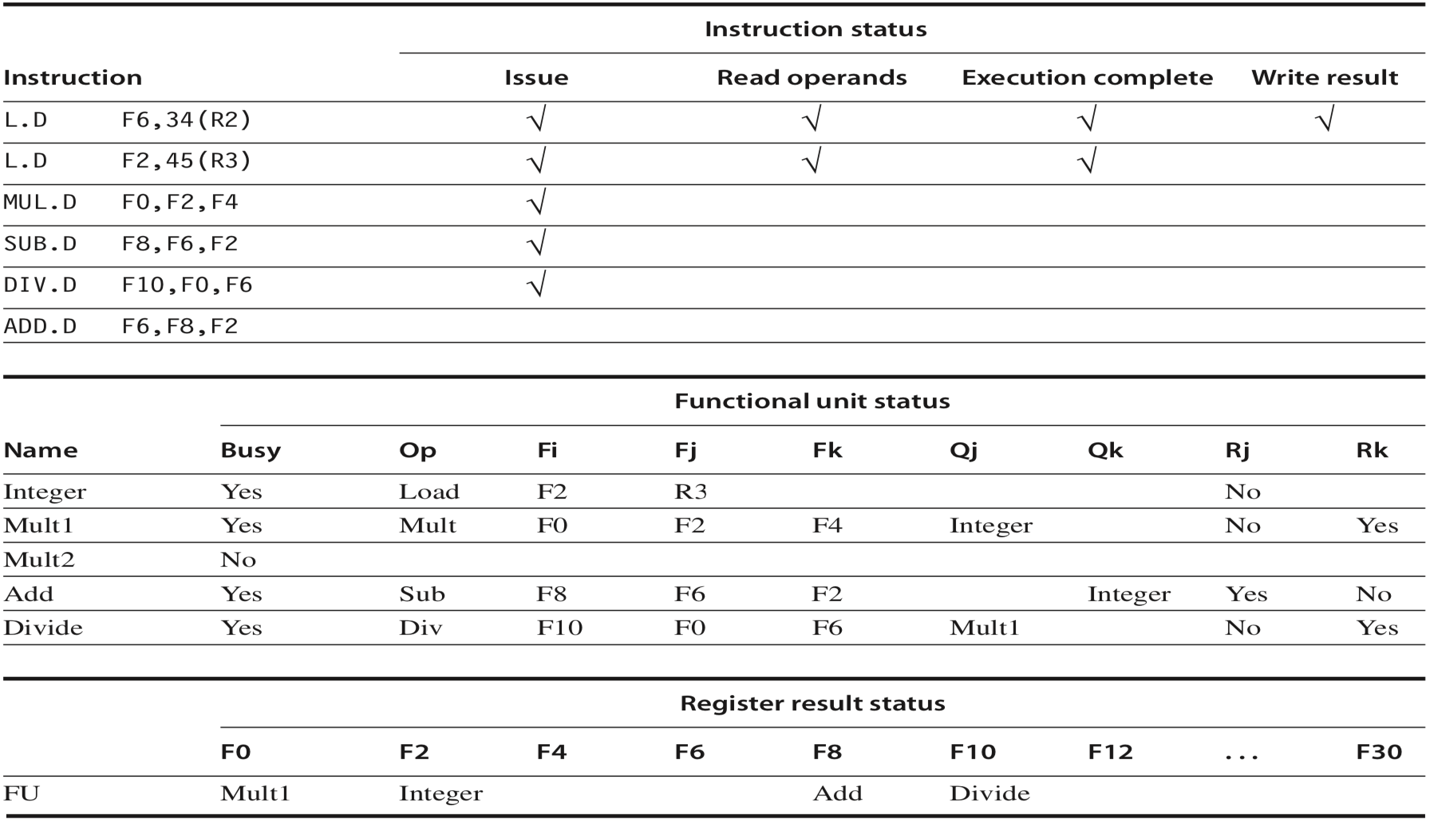
\includegraphics[width=0.42\textwidth]{pic/CA3/Scoreboarding Example}
    \caption{Scoreboarding Example}
\end{figure}

Scoreboard controls the instruction progression from one step to the next by communicating with functional units

Three parts:
\begin{itemize}
    \item Instruction status: 
    \subitem Indicate which of the four steps the instruction is in. 
    \subitem Four steps: issue, read operands, execution, write back
    \subitem Omit memory access because the out-of-order focuses more on FP operations
    \item Functional unit status
    \subitem Indicate the state of the functional unit
    \subitem Nine fields per functional unit (FU)
    \begin{figure}[!htb]
        \centering
        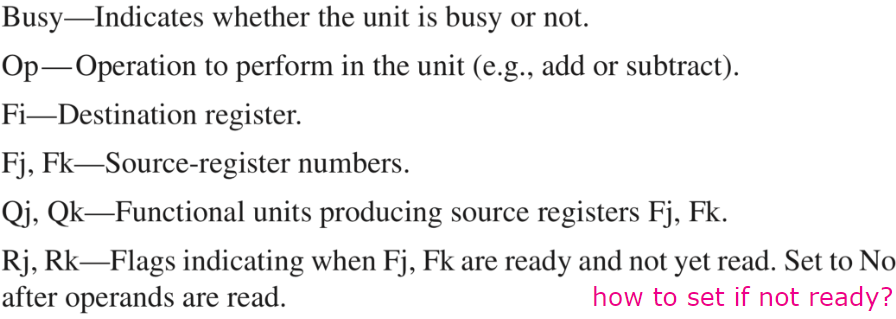
\includegraphics[width=0.42\textwidth]{pic/CA3/Functional Unit Status}
        \caption{Functional Unit Status}
    \end{figure}
    \item Register result status
    \subitem Indicate which functional unit will write each register, if an active instruction has the register as its destination.
    \subitem Set to blank whenever no pending instructions will wirte that register
\end{itemize}
其监控全局信息, 以支持乱序执行. 但当结构过大布线就十分困难, 有单点失效的问题, 有性能瓶颈. 

\subsubsection{Register Renaming}
Elimination of stalls for WAW and WAR hazards through Register Renaming. Rename related destination registers. 


\begin{minted}{text}
    fdiv.d f0, f2, f4           fdiv.d f0, f2, f4
    fadd.d f6, f0, f8           fadd.d S, f0, f8
    fsd    f6, 0(x1)       ->   fsd    S, 0(x1)
    fsub.d f8, f10, f14         fsub.d T, f10, f14
    fmul.d f6, f10, f8          fmul.d f6, f10, T
\end{minted}

\begin{itemize}\scriptsize
    \item RAW(Read after Write) Hazard: no rename
    \item WAR(Write after Read) Hazard: rename latter/destination
    \item WAW(Write after Write) Hazard: rename former
\end{itemize}
after rename destination, rename later source. 如此, 便支持了更大范围的乱序执行. 


\subsubsection{Tomasulo's Algorithm}
\begin{figure}[!htb]
    \centering
    \includegraphics[width=0.309\textwidth]{pic/CA3/Tomasulo’s Algorithm}
    \caption{Tomasulo's Algorithm}
\end{figure}


\begin{itemize}
    \item 用 Reservation stations 存储并等待相关 functional unit 的信息. 对于一条指令, 需要等待其 source register 都 ready, 且 functional unit 完成当前的操作. 
    \item 用 Common data bus (CDB) 链接 functional unit 输出的信息. 需要链接到 register, forwarding, memory. 
\end{itemize}

Two major advantages over scoreboard:
\begin{enumerate}\scriptsize
    \item Distribution of hazard detection logic
    across load/store buffers and
    reservation stations
    \item Elimination of stalls for WAW and WAR
    hazards through Register Renaming
\end{enumerate}

\begin{figure}[!htb]
    \centering
    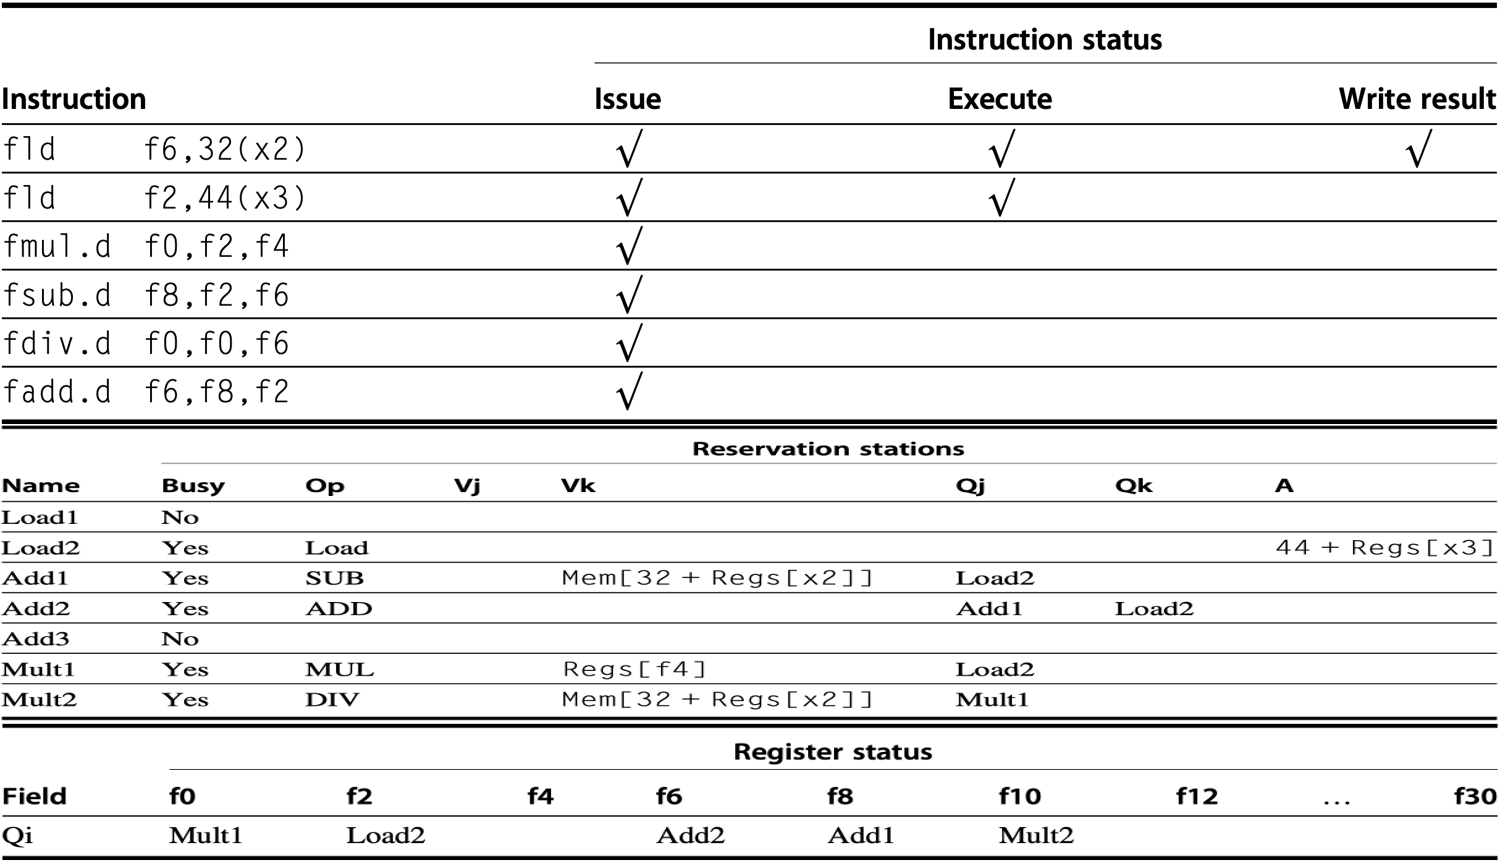
\includegraphics[width=0.42\textwidth]{pic/CA3/Tomasulo Example}
    \caption{Tomasulo Example}
\end{figure}



\subsubsection{Hardware Speculation}
out-of-order execution \& in-order commit and issue
\begin{itemize}
    \item Instruction Commit
    \item Reorder Buffer (ROB)
\end{itemize}

\begin{figure}[!htb]
    \centering
    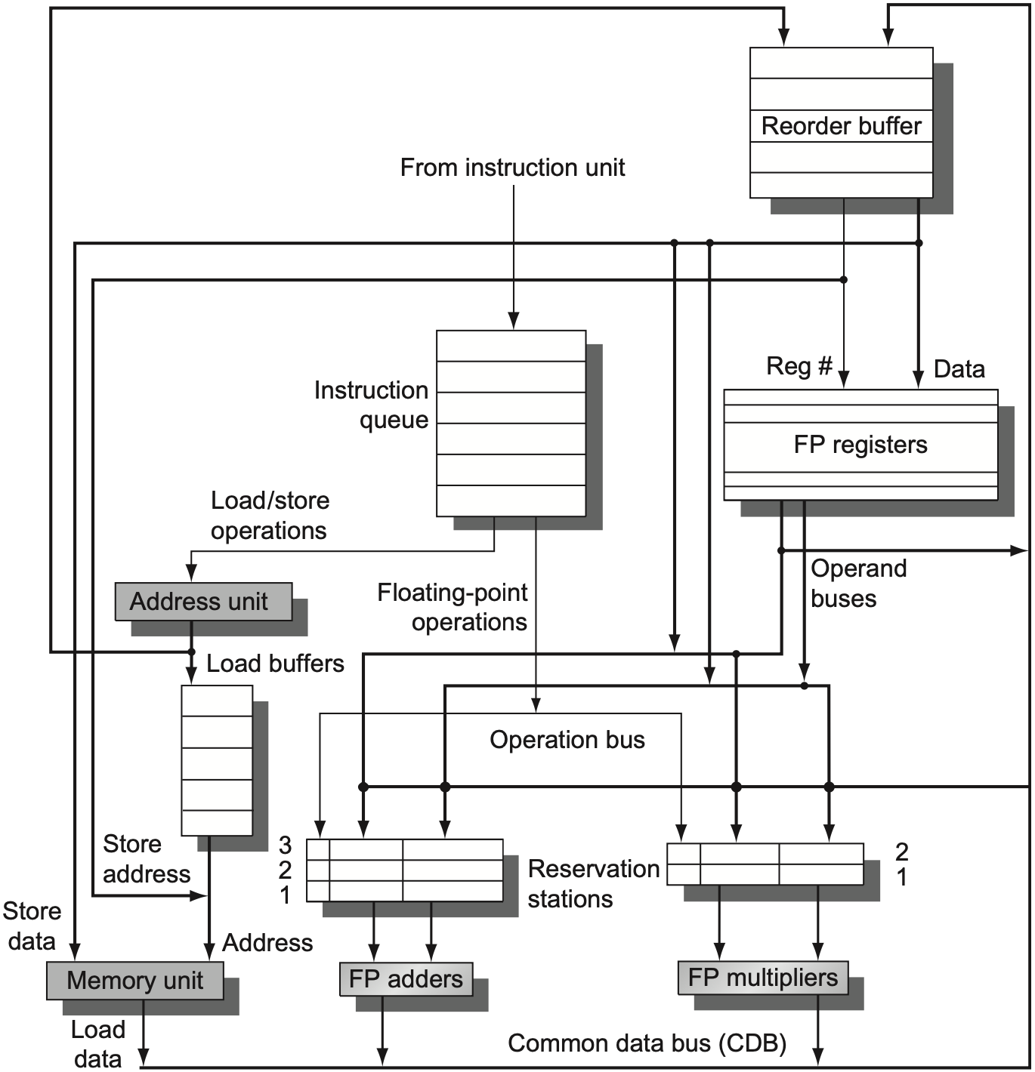
\includegraphics[width=0.309\textwidth]{pic/CA3/Hardware Speculation}
    \caption{Hardware Speculation}
\end{figure}

Reorder buffer 顺序与 instructions 的顺序一致. 若 branch 预测错误, flush Reorder buffer 的相关内容. 

\subsection{Hardware Speculation}
%TODO

\begin{table}[!htb]
    \centering
    \caption{Example}
    \begin{tabular}[c]{ccllll}\toprule
        inst & operand & issue & exe & write & commit \\ \midrule
        div & x2, x3, x4 &  1 &  2 & 42 & 43 \\
        mul & x1, x5, x6 &  2 &  3 & 13 & 44 \\
        add & x3, x7, x8 &  3 &  4 &  5 & 45 \\
        mul & x1, x1, x3 & 14 & 15 & 25 & 46 \\
        sub & x4, x1, x5 & 15 & 26 & 27 & 47 \\
        add & x1, x4, x2 & 16 & 43 & 44 & 48 \\
        \bottomrule
    \end{tabular}
\end{table}

Example: 
\begin{itemize}\scriptsize
    \item free reservation station on result broadcast (not instruction dispatch); 
    \item issue, capture, dispatch in same cycle; 
    \item 1-cycle add, 10-cycle mul, 40-cycle div;
\end{itemize}

exe 是开始执行, write 是执行完 broadcast 的周期, 执行完是在 write-1 的周期. 对于此题, reservation station 只有在 broadcast 后 free, 所以 issue 要推迟. 


\newpage
\section{ILP -- Exploitation}%TODO 
Ideal IPC \& more Data path >1

\subsection{Multiple Issue}

\subsection{VLIW}

\subsubsection{VLIW Scheduling}

\subsection{issue speculation}
Further Example x2


\subsection{Branch-Target Buffer}


\subsection{Return Address Stack}
